%! TEX root = ../thesis.tex

\chapter{The Pierre Auger Observatory}
\label{chap:auger-observatory}

Located on the argentinian high-plains of Pampa Amarilla, the Pierre Auger observatory is a hybrid detector designed to detect and study cosmic 
rays of the highest energies. With an effective area of \SI{3000}{\kilo\meter\squared} it is by far the largest experiment of its kind 
\cite{DesignReport}.

Altough first proposed in 1992, it took 18 years until the idea of a large scale experiment to detect cosmic rays matured and construction of the 
first prototype started near Mendoza \cite{AugerTimeline}. Some further 20 years later, the Pierre Auger collaboration has co-authored over \TODO
publications and continues to advance research in astroparticle physics.

It does this via a hybrid approach, combining measurements of a \textbf{S}urface \textbf{D}etector (SD) as well as a \textbf{F}louresence \textbf{D}etector (FD). 
Additional machinery, such as the e\textbf{X}treme (XLF) and \textbf{C}entral \textbf{L}aser \textbf{F}acility (CLF), is installed to monitor atmospheric 
variables. This improves the overall systematic accuracy of predictions made by the experiment. An overview of the site can be seen in \autoref{fig:auger-array}. 
Data measured by the FD, SD and the atmospheric monitors is sent to a \textbf{C}entral \textbf{D}ata \textbf{A}cquisition \textbf{S}ystem (CDAS) located in the 
nearby town of Malargüe.

This chapter offers a brief look into the measurement principle and setup of the observatory. Information regarding the fluoresence detector can be 
found in \autoref{sec:fluoresence-detector}. The SD is described in \autoref{sec:surface-detector}. A more in depth read on detector specifications 
and design choices is represented by the Pierre Auger observatory design report \cite{DesignReport}, where a lot of information stated in this chapter
is conglomerated from. Notes on the event reconstruction are listed in \autoref{sec:event-reconstruction} and summarized from \cite{SDReconstruction} 
and \cite{FDReconstruction}.

\begin{figure}
	\centering
	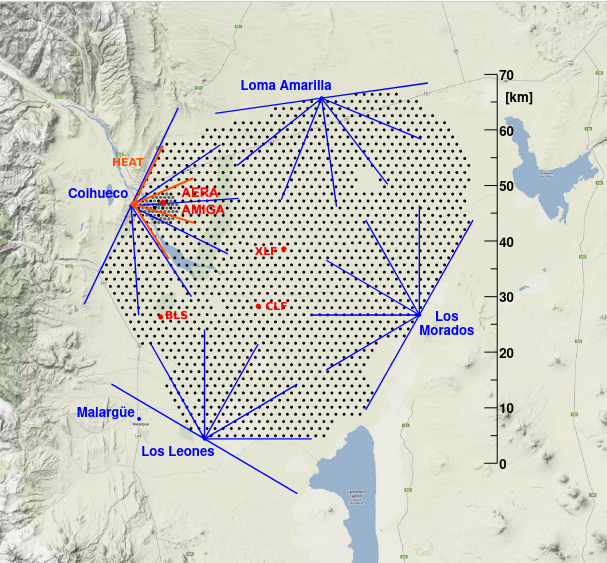
\includegraphics[width=0.9\textwidth]{imgs/auger_array.png}
	\caption{Overview of the Pierre Auger observatory. The four different FD sites (respective FOV shown with blue lines) sit at the edge of
	the detector area and monitor the night sky above the SD array consisting of 1600 water tanks (black dots). A denser spacing of stations 
	near Coihueco is equipped with additional electronics such as e.g. radio antennas (AERA) and muon detectors (AMIGA). Image taken from \cite{AugerArray}}.
	\label{fig:auger-array}
\end{figure}

\section{Fluoresence Detector (FD)}
\label{sec:fluoresence-detector}

The FD consists of a total of 27 fluoresence telescopes (eyes) at 4 different sites. Each eye monitors a \SI{30}{\degree} x \SI{30}{\degree} window 
of the sky at a resolution of $\approx \, 0.5 \, \frac{ \text{px} }{ \text{deg}^2 }$. This results in an effective FOV of roughly \SI{180}{\degree} x 
\SI{30}{\degree} per FD station, with an exception of Coihueco, where three additional telescopes - HEAT (\textbf{H}igh \textbf{E}levation 
\textbf{A}uger \textbf{T}elescope) - are installed to enable monitoring of higher zenith angles ($\SI{30}{\degree}\leq\theta\leq\SI{60}{\degree}$) and
increase sensitivity for showers of lower energies (compare \autoref{chap:physical-background}).

The individual telescopes consist of \SI{3.6}{\meter} by \SI{3.6}{\meter}, convex mirrors. They reflect incoming light onto a set of 440 
photomultipliers (PMTs), each corresponding to one pixel in the resulting image seen by an eye. Since the setup needs to be extremely sensitive to 
UV light in order to detect flouresence caused by extensive air showers, its operation is limited to the relatively noise free moonless astronomical 
nights (Sun $\measuredangle$ Horizon $\lesssim-18^{\circ}$). When the FD is operational, this allows the observation of the longitudinal propagation of 
a shower instead of just its' footprint (as seen by the SD). 

\section{Surface Detector (SD)}
\label{sec:surface-detector}

\TODO PICTURE!

The SD consists of 1600 individually operating stations, spaced apart on a hexagonal grid with a standard \SI{1.5}{\kilo\meter} spacing. Each 
station is made up of a main tank filled with \SI{12000}{\litre} of purified water and reflective inner walls, a solar panel and batteries for power management, 
as well as an antenna for communication. Within each tank three PMTs detect Cherenkov light originating from shower particles, these are together with the tank 
referred to as \textbf{W}ater \textbf{C}herenkov \textbf{D}etectors (WCDs). With the (at the time of this work) ongoing AugerPrime upgrade, each station is 
additionally equipped with a \textbf{s}mall \textbf{PMT} (sPMT), \textbf{S}urface \textbf{S}cintillator \textbf{D}etector (SSD), and radio antenna atop the tank.
This allows for the recording of stronger signals, finer separation of electromagnetic and muonic shower component and detection of highly inclined air showers 
respectively \cite{AugerPrime, horandel2020precision}. 

\subsection{Data acquisition (DAQ)}
\label{ssec:sd-daq}

Onboard electronics, the \textbf{U}pgraded \textbf{U}nified \textbf{B}oard (UUB), or more precisely six 10-bit \textbf{F}lash 
\textbf{A}nalog-to-\textbf{D}igital-\textbf{C}onverters (FADCs) read out measurement data from the PMTs at a sampling rate of \SI{120}{\mega\hertz} 
($\approx\SI{8.33}{\nano\second}$ binning) \cite{verzi2013energy}. This is done in a two-fold way. Three FADCs digitize the PMTs dynode voltage, resulting in the
\textbf{H}igh\textbf{G}ain (HG) output. Three FADCs monitor the anode voltage to form the \textbf{L}ow \textbf{G}ain (LG) output, which can be analyzed if the 
HG output exceeds a value of $2^{10}$ ADC counts and becomes saturated. This effectively enables the measurement of both large ($\geq\mathcal{O}(10^3)$ particles
hitting the tank) as well as small shower signals ($\mathcal{O}(1)$ particle hitting the tank) with sufficient accuracy. Once an FADC bin has been recorded and 
checked for possible triggers (c.f. \autoref{ssec:sd-triggers}) it is written to a ring buffer. If a trigger is issued, the corresponding chunk in the ring 
buffer ($\approx\SI{4.992}{\micro\second}$ (599 bins) before and $\SI{12.07}{\micro\second}$ (1448 bins) after a trigger, $2047 + 1$ bins total), the measured trace, 
can be analyzed in order to calibrate a station in the array (\autoref{ssec:sd-calibration}) or processed by a higher-level CPU for event reconstruction purposes 
(see \autoref{sec:event-reconstruction}).

\subsection{Calibration}
\label{ssec:sd-calibration}

While each station is equipped with the same electronics and runs the same analysis software, variables like the position in the field, station age or slight 
changes in the manufacturing/installation process cause different stations to age differently. Over the lifetime of the array such differences can sum into 
potentially drastic discrepancies in gathered data. Put simply, an extensive air shower will look different both to different WCDs at the same time as well as 
the same WCD at different times. To account for this, measurements are standardized across all stations. ADC counts are related to a \textbf{V}ertical 
\textbf{E}quivalent of through-going \textbf{M}uons (VEM) that would result in the same signal strength. In this fashion, the maximum response that is generated 
by a PMT from one vertically through-going muon is defined as \SI{1}{\Peak}. The total deposited charge (equivalent to the integral of the response) is defined 
as \SI{1}{\Charge}. The conversion factor between ADC counts and VEM$_\text{Peak}$ and VEM$_\text{Ch.}$ is estimated from data and continuously updated separately
for each station. Note that due to the limited computational resources of the WCD, a simplified, rate-based approach is chosen for calibration in the field (Online
algorithm), this stands in contrast to the more physics-driven methods used during event reconstruction (Oflline algorithm). In any case, both algorithms are 
listed in the following subsections and discussed in more detail in the referenced literature.

\subsection{Online algorithm}
\label{ssec:online-calibration}

\TODO Baseline

Once the baseline 


\subsection{Offline algorithm}
\label{ssec:offline-calibration}

\subsubsection{Baseline estimation}
\label{sssec:offline-baseline-estimation}

For event reconstruction, a first baseline estimate of a WCD PMT is predicted by examining the beginning and end of a 2048 bin ($\SI{17.06}{\micro\second}$) long 
trace. The mode $m$ as well as standard deviation $\sigma$ of the first (last) 300 bins is calculated. All bins larger or smaller than $m\pm2\sigma$ are truncated 
and removed from the trace window. The value of $m$, $\sigma$ is consequently updated and the procedure repeated until a convergence is reached and no further cut 
is necessary. The best estimate $B_\text{front}$ ($B_\text{end}$) for the front (end) of the trace at this point is given by the mean value of all remaining bins. 
It's statistic uncertainty $\sigma_{B_\text{front}}$ ($\sigma_{B_\text{end}}$) is given by the standard deviation of the remaining bins \cite{tobiasBaseline}. The 
baseline between the flat front and end estimate is then interpolated based on the difference $\Delta B = B_\text{end} - B_\text{front}$.

\begin{itemize}
	\item \textbf{Rejection of anomalous upward fluctuations} $\mathbf{\frac{\Delta B}{\sigma_{\Delta B}} \geq +10}$:

	$B_\text{end}$ being higher than $B_\text{front}$ often indicates errors in the electronic readout or defect components in the measurement chain. There 
	exists no physical reason why the end baseline should be (significantly) higher than the front. Consequently, traces where this is the case are ignored 
	during event reconstruction.

	\item \textbf{Constant approximation for small upward fluctuations} $\mathbf{+5 > \frac{\Delta B}{\sigma_{\Delta B}} \geq 0}$:

	Small fluctuations of the baseline are expected and the norm. If these fluctuations are positive ($B_\text{end} > B_\text{front}$) the method of 
	calculating the mode, truncating outliers and repeating both steps is applied to the entire length of the signal, resulting in a constant baseline estimate
	$B$ across the trace.

	\item \textbf{Step-function approximation for small downward fluctuations} $\mathbf{0 > \frac{\Delta B}{\sigma_{\Delta B}} \geq -1}$:

	Unlike positive fluctuations, negative fluctuations ($B_\text{end} < B_\text{front}$) can have a physical significance. Due to the undershoof of PMTs after
	detecting a signal in the WCD (compare \cite{glietta2008recovery}), the baseline estimate decreasing towards the end of the trace often indicates the 
	presence of shower particles within the tank. For this reason, downward fluctuations are handled differently from upward ones. If the fluctuations are 
	sufficiently small, the baseline across the trace is estimated as a simple step-function; The trace is separated into two parts along its' maximum ADC 
	value. The front part (i.e. before the max. value) has the baseline $B_\text{front}$, while the rear part is estimated by $B_\text{end}$. An example of 
	this is shown in \autoref{fig:baseline-step-function-approximation}.

	\item \textbf{Charge-linear approximation for large undershoots} $\mathbf{-1 \geq \frac{\Delta B}{\sigma_{\Delta B}}}$:

	For larger undershoots, the baseline is estimated bin by bin based on the deposited charge in the detector. Starting with a value of $B_\text{front}$ for 
	the bins 1-300, the remaining baseline is first linearly interpolated according to \autoref{eq:baseline-charge-linear-interpolation},

	\begin{equation}
	\label{eq:baseline-charge-linear-interpolation}
		b_i = B_\text{front} - \Delta B \cdot \frac{i - 300}{1448}, \qquad 300 \geq i \geq 2048,
	\end{equation}	

	where the magic numbers 300 and 1448 refer to the last bin of the front baseline estimate and the length of the interpolated baseline respectively. From 
	this, the deposited charge $q_i$ up to bin $i$ can be calculated as per \autoref{eq:deposited-charge}.

	\begin{equation}
	\label{eq:deposited-charge}
		q_i = \sum_{k = 0}^{i} \left( T_k - b_k \right)\exp\left(-\frac{\SI{8.33}{\nano\second}}{\tau}\cdot(i-k)\right)
	\end{equation}
	
	In \autoref{eq:deposited-charge}, $T_k$ refers to the numerical value of bin $k$. Note that an exponential falloff term has to be added to account for the
	decay in signal undershoot with a decay time of $\tau = \SI{45}{\micro\seconds}$. The value of $\tau$ is determined in \cite{tobiasBaselineUUB}. Assuming 
	the magnitude of the signal undershoot is directly proportional to the deposited charge $q$, a correction of the baseline thus becomes

	\begin{equation}
	\label{eq:baseline-correction}
		b_i = B_\text{front} + \frac{q_i}{q_{1898}} \cdot \Delta B.
	\end{equation}
	
	The parametrization in \autoref{eq:baseline-correction} is chosen such that the charge-interpolated baseline at bin $1898$ (the center position in the last
	$300$ bins) is exactly equal to the rear baseline estimate $B_\text{end}$. The prediction can be made more accurate by repeating the above steps, each time
	recalculating $q_i$ and readjusting the baseline $b_i$ in the process. \autoref{fig:baseline-charge-linear-interpolation} shows an example baseline 
	estimate after three such iterations. In general, it converges to a robust estimate within five repetitions \cite{tobiasBaselineUUB}.

\end{itemize}

\begin{figure}
	\begin{subfigure}[b]{0.5\textwidth}
		\centering
		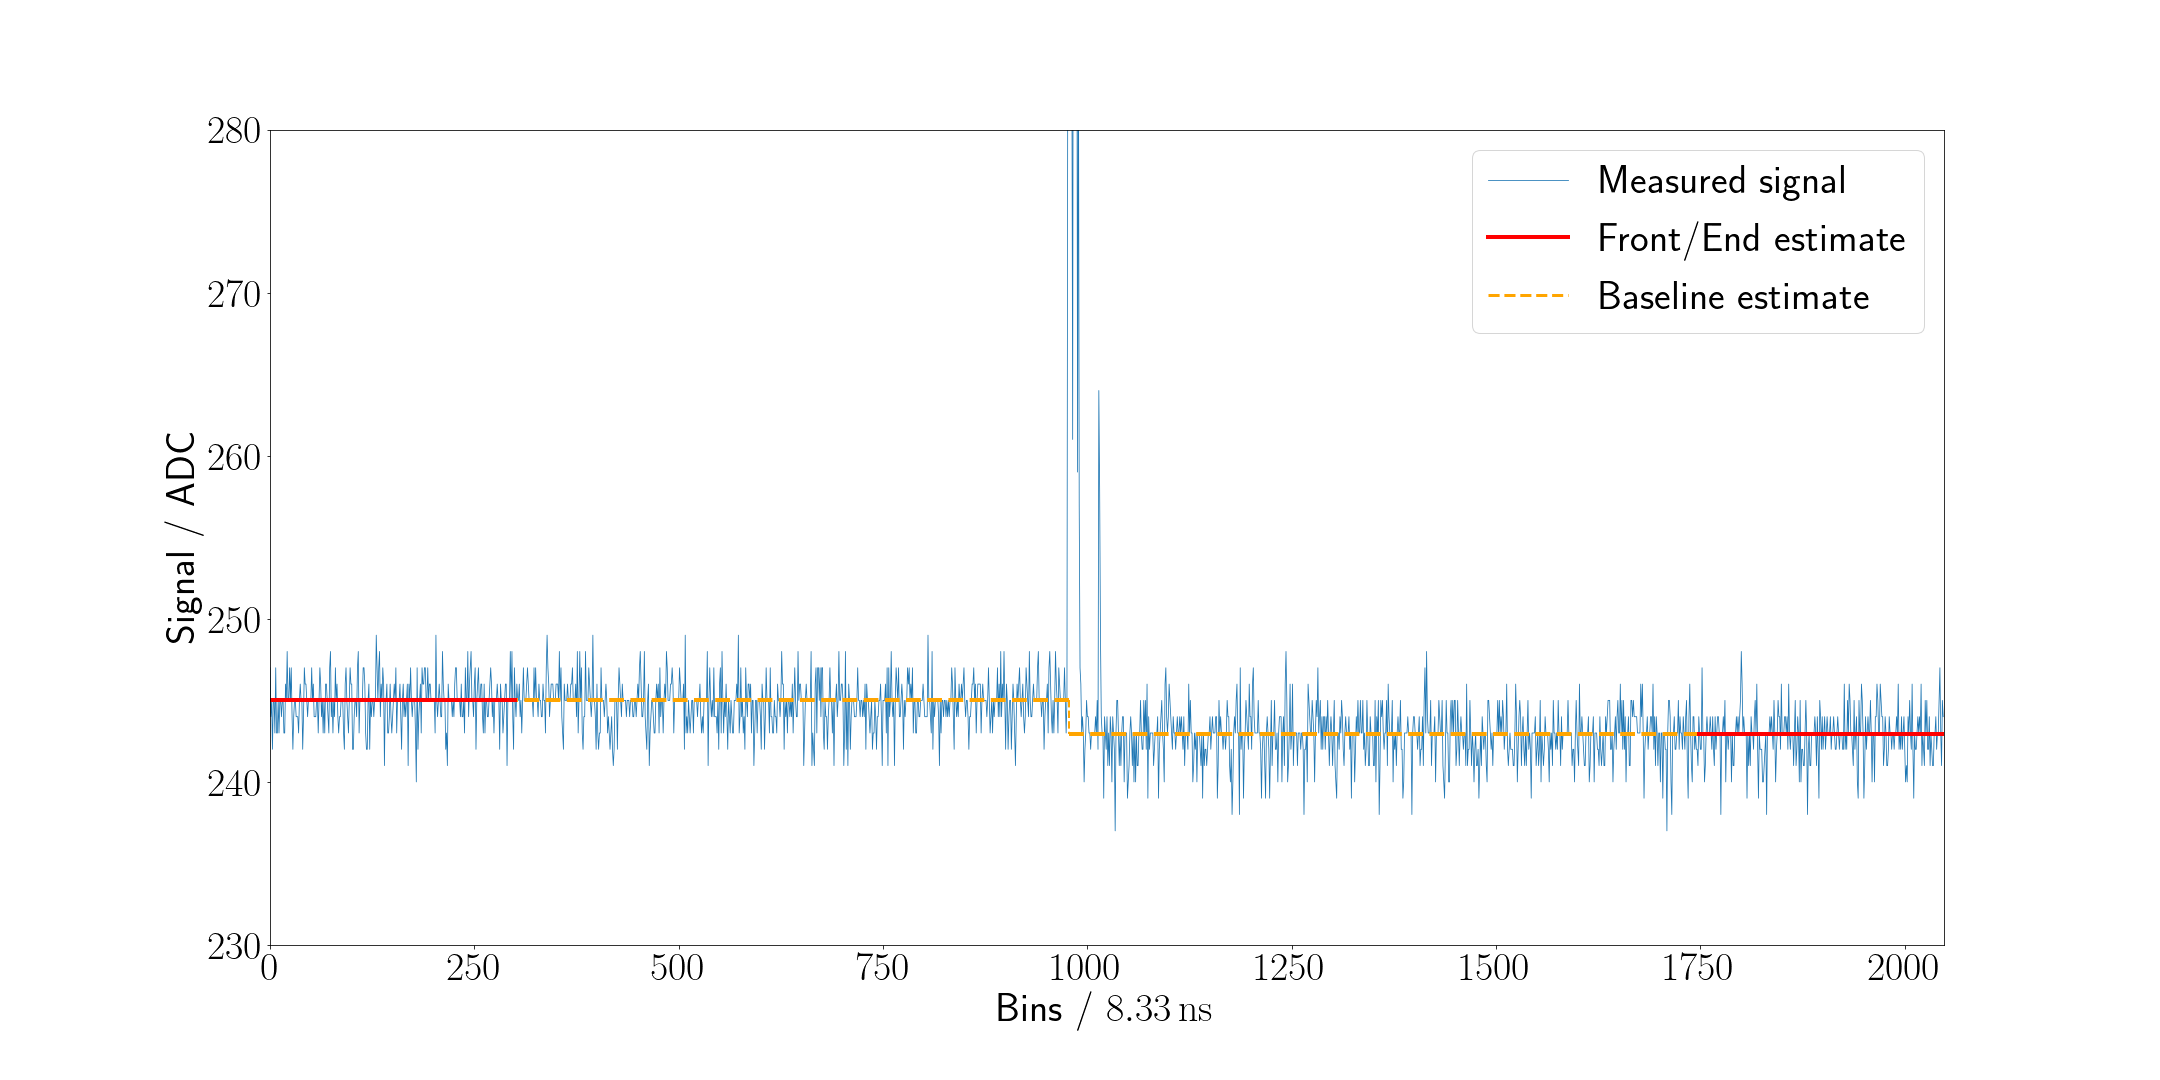
\includegraphics[width=\textwidth]{./plots/baseline_step_function.png}
		\caption{\textbf{Step-function approximation}}
		\label{fig:baseline-step-function-approximation}
	\end{subfigure}
	\hfill
	\begin{subfigure}[b]{0.5\textwidth}
		\centering
		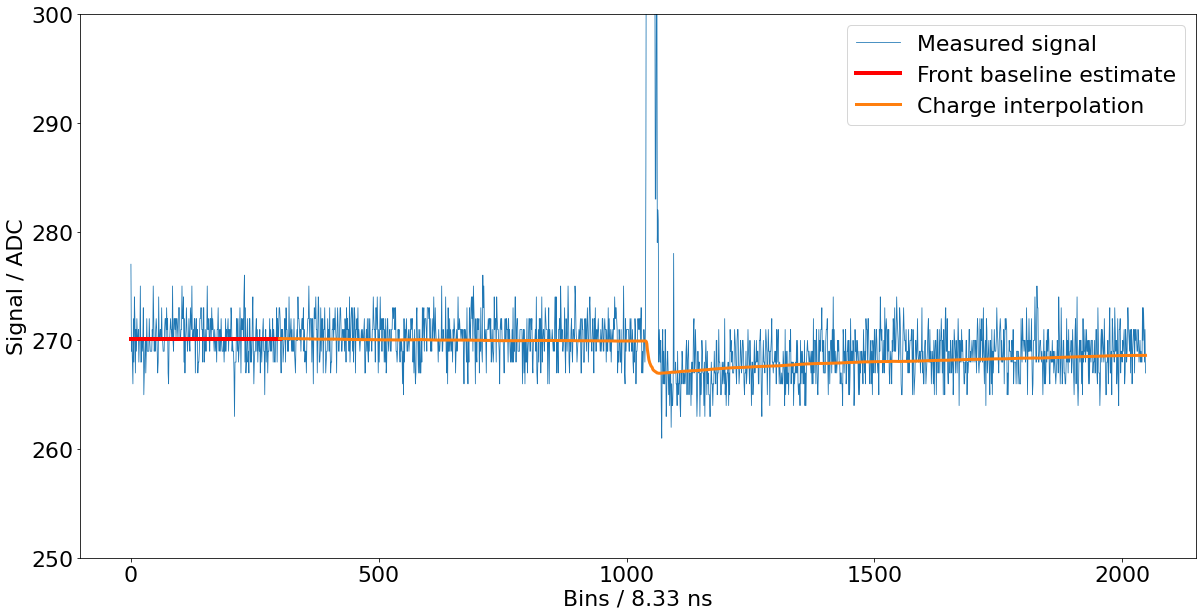
\includegraphics[width=\textwidth]{./plots/baseline_charge_interpolation.png}
		\caption{\textbf{Charge-linear interpolation}}
		\label{fig:baseline-charge-linear-interpolation}
	\end{subfigure}
	\caption{\textbf{(a)} A simple step function is	sufficient to accurately model a PMTs' noise level at small downward fluctuations. \textbf{(b)} For larger 
	discrepancies the more involved charge-linear interpolation is used. Note that the signal undershoot is exaggerated for visualization purposes in both 
	examples.}
\end{figure}

\subsubsection{Estimation of VEM$_\text{Peak}$ and VEM$_\text{Ch.}$}
	\label{sssec:offline-vem-calibration}

The conversion factor between ADC counts and VEM$_\text{Peak}$, VEM$_\text{Ch.}$} are built from distributions of traces that satisfy the muon trigger, which scans
incoming ADC bins for a value exceeding the muon threshold $t_\upmu = b + \SI{30}{\ADC}$, \SI{30}{\ADC} above baseline, for any of the three WCD PMTs. If this 
requirement is met, 69 bins (19 before, trigger bin, 49 after) are written to the muon buffer, a FIFO (first-in-first-out) type memory storage, that is
subsequently filled with low-energy events, which (in general) didn't satisfy any other trigger but still contain useful information.

By histogramming the maximum value (sum) in each trace, a 

\subsection{Trigger procedure}
\label{ssec:sd-triggers}




\section{Event Reconstruction}
\label{sec:event-reconstruction}


